\chapter{Ontologie Computazionali}

\section{Introduzione}

\dfn{Ontologia}{
  Un \newfancyglitter{artefatto di ingenieria} costituito da uno specifico \newfancyglitter{vocabolario} usato per descrivere una certa realtà, aggiungendo un insieme di assunzioni esplicite a proposito del \newfancyglitter{significato inteso} dal vocabolario stesso.
}

\clm{}{}{
  \begin{itemize}
    \item Rappresentazione astratta di concetti e loro relazioni. 
    \item Ontologie formali: rappresentate secondo un formalismo di rappresentazione.
    \item Finalità: condividere una concettualizzazione comune tra individui, organizzazioni, macchine.
  \end{itemize}
}

\paragraph{Elementi costituitivi delle ontologie:}

\begin{itemize}
  \item Classi. 
  \item Proprietà. 
  \item Assiomi. 
  \item Individui.
\end{itemize}

\cor{Ontologie Formali}{
Le ontologie formali si basano su linguaggi
che permettono di descrivere in maniera
esplicita: 
\begin{itemize}
  \item Le caratteristiche delle classi. 
  \item Le caratteristiche delle relazioni tra
classi. 
\end{itemize}
}

\nt{Questi linguaggi permettono alle macchine
di fare inferenze sui concetti e a noi di
avere certezza della validità di queste
inferenze.}

\paragraph{Tipi di ontologie:}

\begin{itemize}
  \item \fancyglitter{Ontologie top-level}: concetti fondazionali comuni a tutti i domini
(spazio, tempo, ecc.).
  \item \fancyglitter{Ontologie mid-level}: utilizzano il livello fondazionale per definire
concetti generali ma non fondazionali: organizzazioni,
comunicazione, stati fisici, sistemi di misurazione, ecc.
  \item \fancyglitter{Domain ontologies}: rappresentano i concetti e le relazioni proprie
di un dominio specifico.
\end{itemize}

\begin{figure}[h]
    \centering
    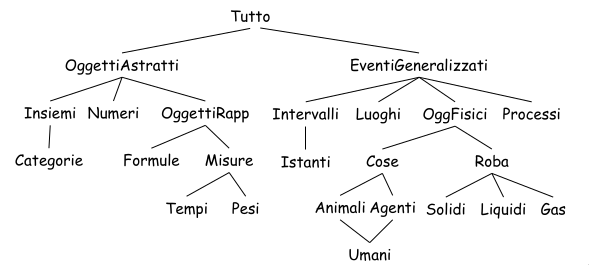
\includegraphics[scale=0.5]{02/Esempio di ontologia top.png}
    \caption{Esempio di ontologia top-level.}
\end{figure}

\subsection{Conoscenza}

\dfn{Conoscenza di Senso Comune}{
La conoscenza di senso comune (commonsense knowledge) è molto
importante per i task che comportano l’interazione con le persone.
}

\nt{Per esempio per chatbot e robot.}

\dfn{CYC}{
  CYC: enCYClopedic Knowledge, conoscenza enciclopedica. Base di conoscenza finalizzata a rappresentare tutto. Comprende oltre 200.000 concetti. 
}

\nt{OpenCyc è la versione open source (quindi superiore), ma non è più disponibile direttamente.}

\clm{}{}{
  \begin{itemize}
    \item La base di conoscenza (Knowledge Base, KB) di CYC
consiste di: 
\begin{itemize}
  \item \fancyglitter{Termini}, il vocabolario di CYC. 
  \item \fancyglitter{Asserzioni} che mettono in relazione questi termini.
\end{itemize}
\item Queste asserzioni includono: 
  \begin{itemize}
    \item Asserzioni semplici. 
    \item \fancyglitter{Regole}.
  \end{itemize}
  \end{itemize}
}

\paragraph{Struttura di CYC:}

\begin{itemize}
  \item La KB di Cyc è divisa in molte \fancyglitter{microteorie} (microtheories),
ciascuna delle quali è costituita da un insieme di asserzioni che
condividono le stesse assunzioni. 
\item Le microteorie si focalizzano su un particolare dominio di conoscenza.
\item Il ragionamento avviene all’interno della singola microteoria. 
\item Questa suddivisione permette al sistema di fare asserzioni che
sarebbero apparentemente contraddittorie.
\end{itemize}

\begin{figure}[h]
    \centering
    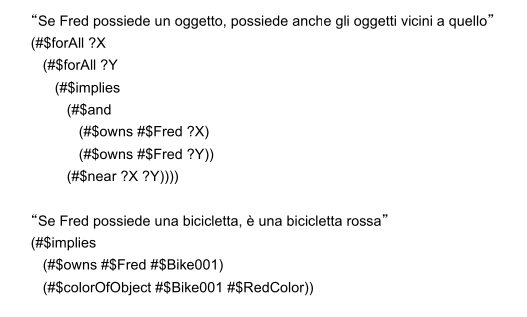
\includegraphics[scale=0.5]{02/rule.png}
    \caption{Esempi di regole.}
\end{figure}

\qs{}{Come ragiona CYC?}

\begin{itemize}
  \item Il \fancyglitter{motore inferenziale} di CYC è in grado di effettuare la
deduzione logica (modus ponens, modus tollens,
quantificazione universale e esistenziale) e i
meccanismi di inferenza tipici dell’IA (ereditarietà,
classificazione automatica).
\item La dimensione della base di conoscenza (200.000
termini e dozzine di asserzioni riguardanti ogni termine)
hanno richiesto la messa a punto di tecniche speciali
per affrontare la complessità.
\end{itemize}

\paragraph{Applicazioni di CYC:}

\begin{itemize}
  \item Modellazione della conoscenza. 
  \item Apprendimento e pattern recognition. 
  \item Assistenti intelligenti. 
  \item Sicurezza delle reti. 
  \item Basi di dati.
\end{itemize}

\dfn{SUMO}{
Ontologia non più mantenuta perché incorporata in altri progetti. 

SUMO (Suggested Upper Merged Ontology) è un'ontologia di alto livello che incorpora un insieme di modelli. È scritta in KIF (Knowledge Interchange Format).
}

\paragraph{SUMO contiene:}

\begin{itemize}
  \item \fancyglitter{Termini}: indivisui e classi, con relazioni gerarchiche (instance e subclass). 
  \item \fancyglitter{Connettivi AND e OR}. 
  \item \fancyglitter{Quantificazione e implicazione}.
\end{itemize}

\clm{}{}{
  \begin{itemize}
    \item Di ogni classe SUMO descrive le caratteristiche attraverso un insieme di assiomi. 
    \item Tali assiomi sono espressi utilizzando le relazioni
contenute nell’ontologia. 
  \end{itemize}
}

\begin{figure}[h]
    \centering
    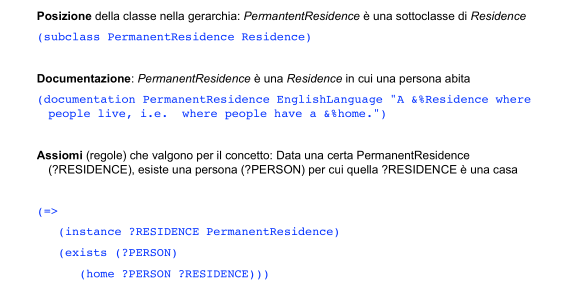
\includegraphics[scale=0.5]{02/sumo class.png}
    \caption{Esempio di classe.}
\end{figure}

\nt{Si possono descrivere relazioni di parti.}

\begin{figure}[h]
    \centering
    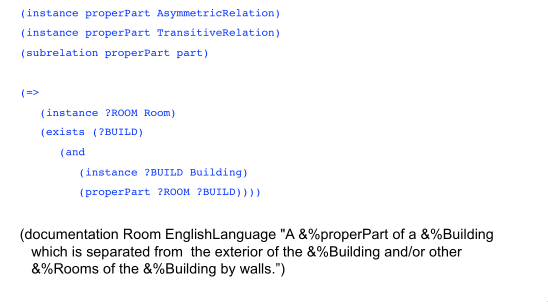
\includegraphics[scale=0.5]{02/partof.png}
    \caption{Esempio di relazione part-of.}
\end{figure}

\nt{Il browser per consultare SUMO si chiama \fancyglitter{Sigma}. No, non metterò un meme brainrot su Sigma.}

\subsection{Altre Ontologie}

\dfn{Ontologie Lightweight}{
Le ontologie leggere sono, normalmente, semplici tassonomie, senza assioni e con poche relazioni. Facilmente standardizzabili.
}

\cor{WordNet}{
Rete di concetti rappresentati da insiemi di termini (detti synset). 
Relazione di sussunzione tra concetti (synset).
}

\dfn{Ontologie Large-Scale}{
  Sono ontologie di grandi dimensioni: 
  \begin{itemize}
    \item Possono essere ottenute tramite l’estrazione automatica di
concetti da testi (Dbpedia e YAGO). 
\item Dall’integrazione di risorse (YAGO e YAGO2) diverse, incluse
risorse lessicali. 
\item Dal lavoro di una comunità di utenti (CYC), via crowd sourcing.
  \end{itemize}
}

\nt{Date le dimensioni, gli strumenti di indicizzazione e di
accesso acquisiscono grande importanza: spesso vengono pubblicate online e come tali integrate in altre
applicazioni.}

\clm{}{}{
  \begin{itemize}
    \item Per l’accesso ai concetti dell’ontologia, è importante l’integrazione
tra di essi e il linguaggio naturale. 
\item L’integrazione avviene: 
  \begin{itemize}
    \item Attraverso la documentazione, cioè associando a ogni concetto
una sua descrizione informale in linguaggio naturale. 
\item Associando ai concetti una entry lessicale in una risorsa
linguistica esterna. 
  \end{itemize}
  \end{itemize}
}

\dfn{DBPedia}{
Iniziativa di ricerca iniziata nel 2007. DBPedia punta a estrarre contenuti strutturali dal progetto wikipedia. DBPedia consente agli utenti di estrarre relazioni e proprietà associate a risorse di wikipedia.
}

\dfn{Linked Open Data}{
  Dati pubblicamente disponibili (Open), pubblicati secondo il paradigma
dei Linked Data. I dataset risiedono nella rete, formando il Linked Open Data (LOD) Cloud.
}

\begin{figure}[h]
    \centering
    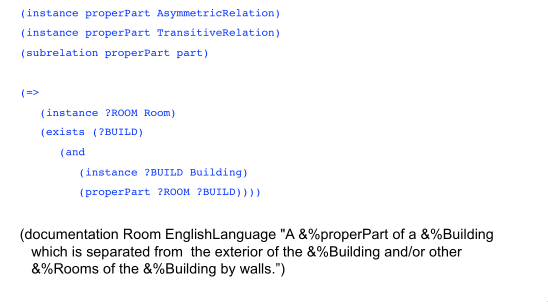
\includegraphics[scale=0.5]{02/partof.png}
    \caption{Linguaggi per descrivere ontologie.}
\end{figure}

\subsection{Relazioni tra Classi}

\dfn{Sottoclasse}{
  Tutti gli elementi della sottoclasse
sono elementi della (sovra)classe,
ma non viceversa. 
}

\cor{Classi Disgiunte}{
  Due classi sono disgiunte se non hanno
elementi in comune.
}

\begin{figure}[h]
    \centering
    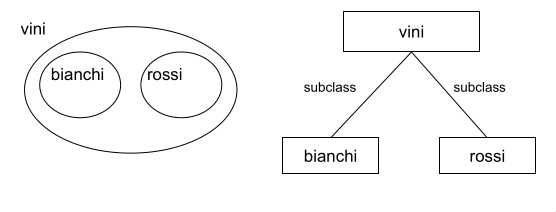
\includegraphics[scale=0.6]{02/classdisg.png}
    \caption{Esempio di classi disgiunte.}
\end{figure}

\cor{Scomposizione Esaustiva}{
Due o più classi sono scomposizione esaustiva
di una classe se tutti gli elementi della classe
appartengono a una di esse
}

\nt{\{Statunitensi, Canadesi, Messicani\} sono la
scomposizione esaustiva di Nordamericani\footnote{Trump non approva questo elemento, è palese che il Canada sia il 51°esimo stato}.}

\cor{Partizione}{
  Scomposizione esaustiva con classi disgiunte.
}

\begin{figure}[h]
    \centering
    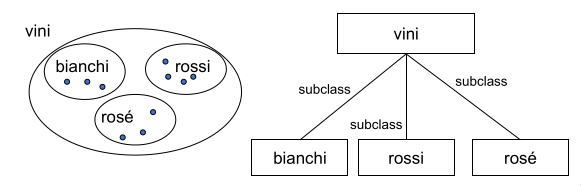
\includegraphics[scale=0.6]{02/partizioni.png}
    \caption{Esempio di partizione.}
\end{figure}

\dfn{Logiche Descrittive}{
  Le logiche descrittive sono:
  \begin{itemize}
    \item Orientate alla classificazione. 
    \item Basate sulla relazione di sottoclasse (sussunzione). 
    \item Completezza e trattabilità computazionale. 
    \item Sono la base del Progetto Web Semantico.
  \end{itemize}
}

\clm{}{}{
  \begin{itemize}
    \item Nelle logiche descrittive si distinguono le definizioni di concetti
dalle asserzioni sugli individui fatte utilizzando quei concetti: 
\begin{itemize}
  \item \fancyglitter{T-Box}: Terminologia, cioè definizione di concetti generali.
  \item \fancyglitter{A-Box}: Asserzioni su singoli individui. 
\end{itemize}
  \end{itemize}
}

\dfn{Ruoli}{
  \begin{itemize}
    \item I ruoli costituiscono il mezzo per
mettere in relazione i concetti. 
\item In CLASSIC, il predicato che
permette di esprimere il concetto
di ruolo è FILLS. 
\item Tipicamente, si possono porre
restrizioni numeriche sui ruoli
(Atleast, Atmost). 
\item Un motore inferenziale (reasoner)
usa queste informazioni per
effettuare ragionamenti.
  \end{itemize}
}

\paragraph{Terminologia vs. Asserzioni:}

\begin{itemize}
  \item La terminologia è un insieme di assiomi logici su classi
e proprietà: 
\begin{itemize}
  \item Sussunzione tra concetti (subclass). 
  \item Relazioni generiche in cui gli elementi di determinate classi
rivestono un ruolo.
\end{itemize}
\item Data la terminologia, si fanno asserzioni su un insieme
di individui. 
\begin{itemize}
  \item Le asserzioni devono essere coerenti con la terminologia (non
si può dire che uno scapolo è sposato). 
\end{itemize}
\end{itemize}

\qs{}{
  Cosa si chiede a un sistema basato su DL?
}

\begin{itemize}
\item \fancyglitter{Instance checking}: verificare se un
certo individuo (nella A-Box)
appartiene a una classe. 
\item \fancyglitter{Relation checking}: verificare se vale
una certa relazione tra classi.
\item \fancyglitter{Subsumption}: verificare se una classe
è un sottoinsieme di un'altra classe.
\item \fancyglitter{Concept consistency}: verificare che le
definizioni e le loro conseguenze non
siano contraddittorie.
\end{itemize}













